\begin{figure}
  \ContinuedFloat*
  \begin{tabular}[t]{c c}
    \begin{minipage}{0.5\textwidth}
      \begin{Verbatim}[mathescape,commandchars=\\\{\}]
\textbf{let} s = stim 2 \textbf{in}
  \textbf{let} p = pop 2 1 \textbf{in}
    s $\otimes$ p
      \end{Verbatim}
    \end{minipage} & \begin{minipage}{0.5\textwidth}
      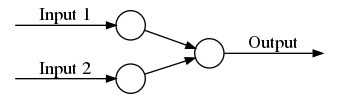
\includegraphics[width=\textwidth]{chapters/volr/example1.pdf}
    \end{minipage}

  \end{tabular}
  \caption{A textual and visual example of a network with a stimulus,
    a population and an implicit output.}
  \label{fig:volr-example1}
\end{figure}

\begin{figure}
  \ContinuedFloat*
  \begin{tabular}[t]{c c}
    \begin{minipage}{0.5\textwidth}
      \begin{Verbatim}[mathescape,commandchars=\\\{\}]
\textbf{let} s = stim 2 \textbf{in}
  \textbf{let} p = pop 2 1 \textbf{in}
    s $\otimes$ p
      \end{Verbatim}
    \end{minipage} & \begin{minipage}{0.5\textwidth}
      Hello
    \end{minipage}
  \end{tabular}
\label{fig:volr-examples}
\end{figure}